% Chapter Template

\chapter{Product Design} % Main chapter title

\label{Chapter2} % Change X to a consecutive number; for referencing this chapter elsewhere, use \ref{ChapterX}

App design combines User interface (UI) and User Experience (UX), while UI is concerned about how the app pages look like and feel, such as the fonts, colours and arrangements of icons, UX focuses on the functionality and usability. The best app design process comprises research, 
ideation, problem identification, design, feedback and problem evaluation. Currently, we only focus on the mobile app design or specifically IOS design based on Apple Platform and Android Design. 
%-----------------------------------------------------------------------------------------------------------------------------UX
\section{UX Design}
UX Design is the process of deciding how someone will use an app and creating a viable product. It’s during the UX process that mobile app design ideas are generated and validated, to make sure that all your choices are going to work so that our app works. 
\\The quality of user experience is the crucial factor in measuring the quality of the design and usually it's the key to distinguishing a successful app design from an unsuccessful one. 
Customers are becoming pickier about which app to use and so quick to abandon the app which they do not enjoy, so it's essential to invest time and effort in creating a great user experience.
\subsection{Minimum Viable Product (MVP)}
A minimum viable product, or MVP,  is a product with enough features to attract early-adopter customers and validate a product idea early in the development cycle. To decide which features belong to the MVP design, we use the MoSCoW method to represent all the features we want to include in our design, which are M (Must Have) o S (Should Have) C (Could Have) o W (Won’t Have). 
The table separates the features for our MVP from the advanced functions that we want to include in our design.

\begin{table}[ht]
\centering
\begin{tabular}{ |c|c| } 
 \hline
\textbf{MUST HAVE FEATURES FOR MVP} & \textbf{SHOULD/ COULD HAVE FEATURES}\\ 
 \hline
 Sign-up and sign-in with email & Sign-in with third party accounts \\ 
 \hline
 Upload Audio & Real-time generation \\ 
 \hline
 Chord output & Chord regeneration \\ 
 \hline
 Chord layout &  Export to PDF \\ 
 \hline
 Share posts & Message channel \\ 
 \hline
 Recommendation Engine &  Lock Chords when regenerating\\ 
 \hline
 Help and support &  Pitch Tracking\\ 
 \hline
 File storage& File backup \\ 
 \hline
 \end{tabular}
 \caption{MoSCoW Table}
 \centering
 \end{table}
 
 \subsection{User Flow and Funtionality}
User flows are flowcharts that illustrate the movement or journey of a user through your app. User flow diagrams are indispensable in mastering user experience. 
They allow us to understand how users interact with our app, and the steps they take to complete a task or achieve a goal on our app. This will help us create a superior user experience for the user and meet their needs more efficiently.  
\\One of our user flow examples is shown in Figure:\ref{flowchartmain}
We use a rounded rectangle to represent the termination, a diamond to represent the decision, a rectangle to represent the process and an arrow to represent the flow direction.

\begin{figure}[ht]
\centering
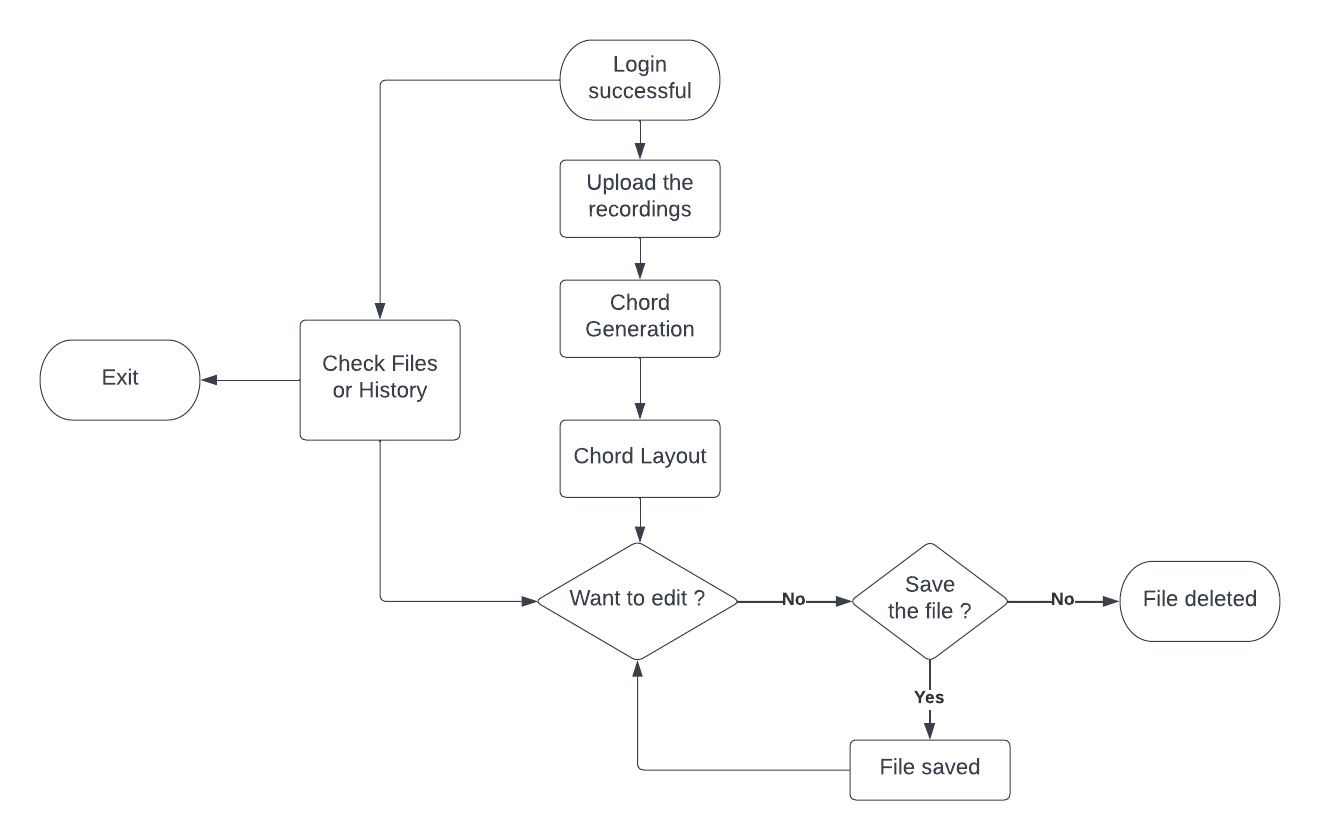
\includegraphics[scale = 0.25]{MFpage.png}
\caption{User Flow Diagram for main function page}
\label{flowchartmain}
\end{figure}


\subsection*{Main Functionality}

\begin{itemize}

\item \textbf{Sign-up and Sign-in with Email}
\\From the start, our users can sig-up with their email and then login in with our app accounts. The reason why we want our users to create an account is that we can profile our users more easily.

\item \textbf{Sign-in with with third-party Accounts}
\\ The purpose is to reduce the barriers for our users to enter our app. OAuth (Open Authorisation) is an open standard for access delegation, commonly used as a way for internet users to grant websites or applications access to their information on other websites but without giving them the passwords. This mechanism is used by companies such as Amazon, Google, Facebook, Microsoft, and Twitter to permit users to share information about their accounts with third-party applications or websites.

\item \textbf{Ask for song tag preference}
\\After our user sign-in, a question with selective answers will show on the main page, the answers will be stored and fed to our recommendation engine \autoref{Content Based Recommendation System}.

\item \textbf{Store and backup files on Cloud}
\\The purpose is to enable better synchronisation between devices and accessibility to the files. 
We will include CloudKit in our IOS design to allow users to store their saved files in iCloud, (merit: grate integration, recordings can also be stored)

\item \textbf{Recording input}
\\ To obtain the audio source, we allow our users to record their singing using our app or upload a previous recording 
from a built-in app such as Voice Memos on iPhone. To fit the audio processing (section:\ref{ssec:crepe}), the recording will be initially sampled at 16hz.

\item \textbf{Chord generation and regeneration}
\\Unlike Chordify, which generates the same chords each time for the same audio source, we provide the option for users to regenerate the chords and we aim to provide sightly different chords when the regeneration button is pressed. 
We will also allow our users to lock the chords they like during the regeneration. \autoref{}

\item \textbf{Community Page}
\\Inspired by the Chinese music app, NetEase, one of our goals is to create a community page for our users to share their works and collaborate, 
we believe that the community element can bring continuous traffic to our app, which can benefit the monetisation of our app in the future.
As we mentioned before, the user experience determines the successfulness of the app design and here the quality of the posts recommended to our users is an important element affecting our user experience. 
Therefore, it requires our recommendation engine to be well designed. Chapter\ref{Chapter6}

\item \textbf{Message Channel}
\\The message channel allows our users to contact each other directly and share the original chord files to collaborate on.

\end{itemize}




%-----------------------------------------------------------------------------------------------------------------------------UI
\section{UI Design}
After having the map of user flow, we started to design the prototype using Figma, which is a design tool for prototyping projects. 
There are three example sketches in \autoref{UIdesign}. 

\begin{figure}[ht]
    \label{UIdesign}
     \centering
     \hspace{16mm}
     \begin{subfigure}[b]{0.2\textwidth}
         \centering
         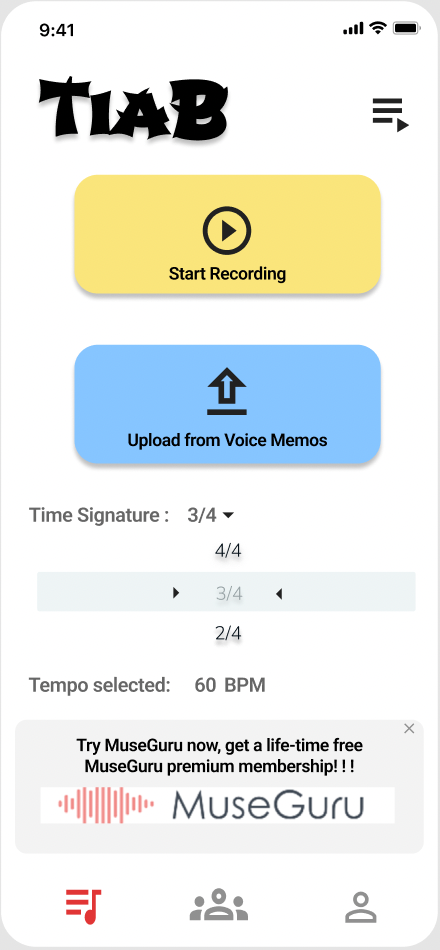
\includegraphics[width=\textwidth]{mianpage1.png}
         \caption{Main page - audio-upload page}
         \label{Mainpage}
     \end{subfigure}
     \hfill
     \begin{subfigure}[b]{0.2\textwidth}
         \centering
         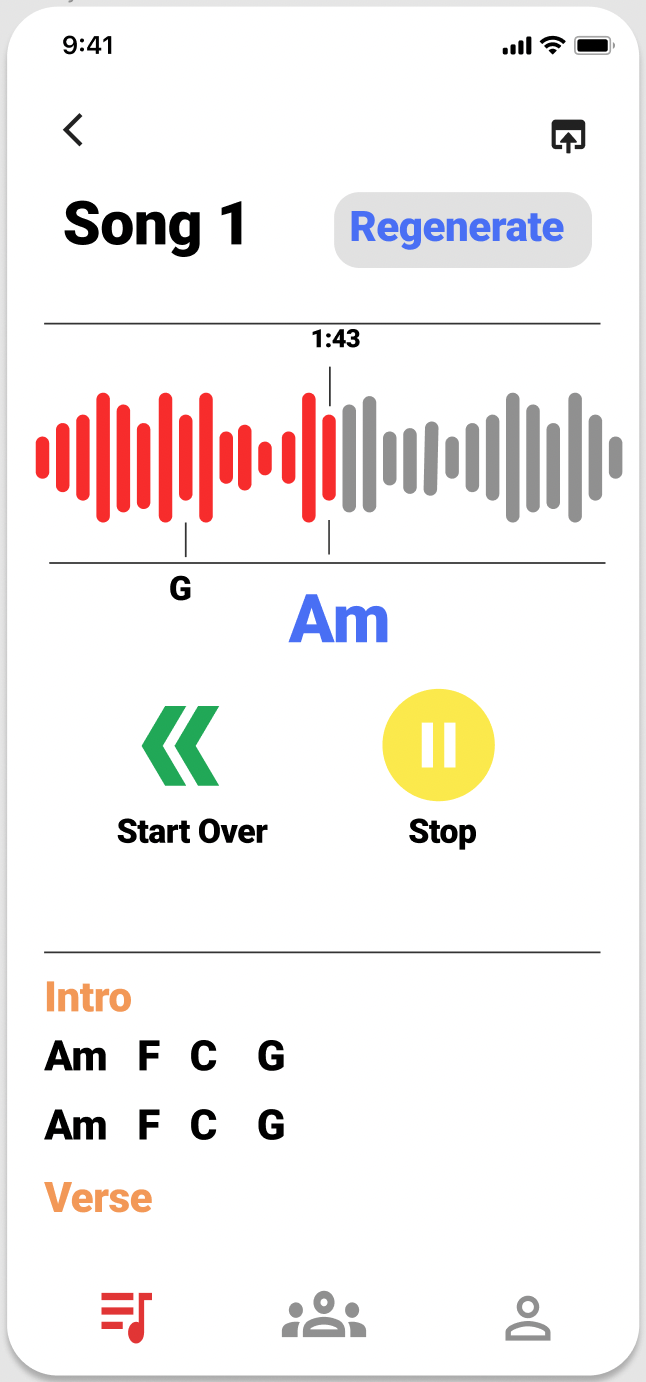
\includegraphics[width=\textwidth]{grappp.png}
         \caption{Chord layout and editting page}
         \label{chordedit}
     \end{subfigure}
     \hfill
     \begin{subfigure}[b]{0.2\textwidth}
         \centering
         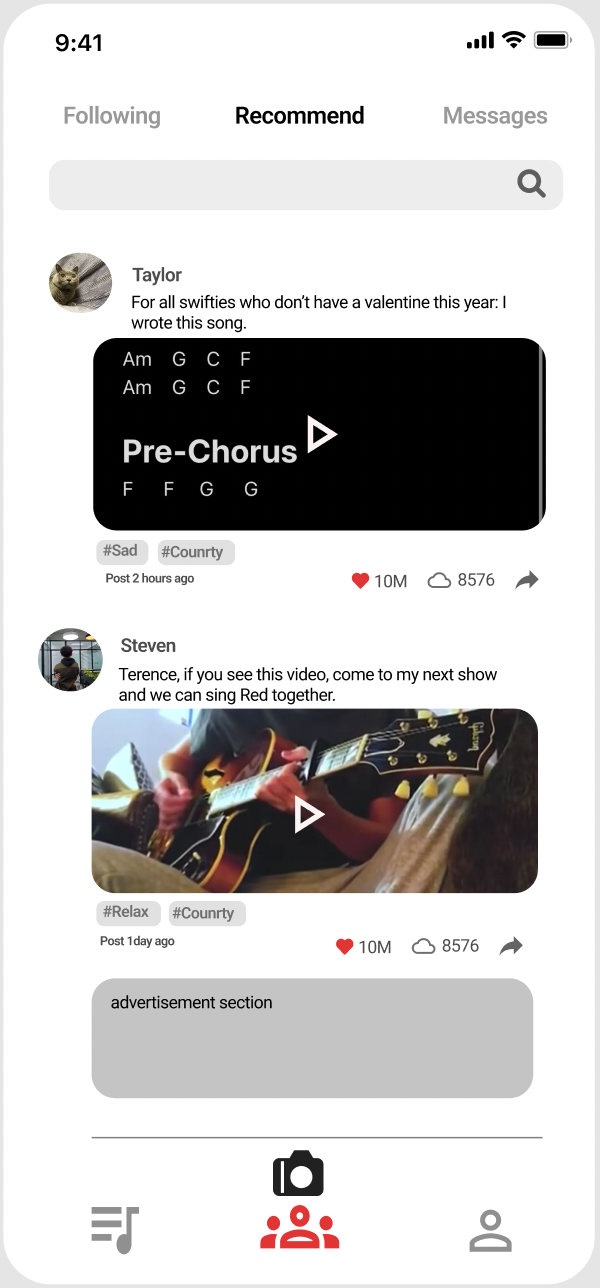
\includegraphics[width=\textwidth]{commupage.png}
         \caption{Community page}
         \label{Community page}
     \end{subfigure}
     \hspace{16mm}
        \caption{UI design for our app}
        \label{fig:three graphs}
\end{figure}

\section{Testing}
The testing stage allows us to discover the problems in our current designs and improve our current designs. 
According to Compuware, 48\% of users are less likely to use an app again if they are troubled with the app’s performance.
As reported by Compuware, only 16\% of users can give the app a try for a second or third time. \footfullcite{lowtole}
\\
We divide our testing stage into four stages, Unit Tests, Integration Tests, System Tests, and Acceptance Tests.
\\\textbf{Unit Test} is the very first stage of any application test. Here, the system’s separate modules will undergo assessments to see if they, individually, function correctly and to maximum capacity. 
\\\textbf{Integration Test}level is mostly about verifying the modules and checking their readiness and their collective, integral cooperation. The modules are each tested separately and also as a group. This aids the testers to identify any issues with two or more components working together or individually to execute functions.
\\\textbf{System Test} level closely simulates the final production environment and is very significant as the final testing stage, especially when it needs to ensure that the applications under scrutiny always meet up to full functional requirements. 
This is where the test team ascertains if the integrated components are collectively showing optimal performance levels or not. For this, every software build must undergo testing up to this point, using client requirements as a benchmark. 
This stage is carried out by the quality assurance engineer in our team.
\\\textbf{Acceptance Test} is the stage where we will include A/B testing in our Beta test. After we have a functionally-reliable version of the app, 
we will be performing A/B testing by providing different UI designs to different groups of test users, this method allows us to 
determine which choice is more attractive.



